\documentclass[10pt,a4paper]{article}
\usepackage[utf8]{inputenc}
\usepackage{ngerman}
\usepackage{graphicx}
\usepackage{amsmath}
\usepackage{amsfonts}
\usepackage{amssymb}


\begin{document}

\title{Technische Dokumentation\\\bigskip
Ubiquitous Computing\\
Team: Ottos }
\author{
Thomas Wiedemann\\ 
Thomas Bargetz\\
Franziskus Domnig\\
Matthias Schmid \\
Florian Gopp\\
Dominik Müller\\ }

\maketitle
\begin{center}
ITM 10\\\bigskip


\end{center}

\newpage
\tableofcontents
\newpage
\section{Projektbeschreibung}
Für das BeagleBoard, bestückt mit einem OMAP3530 von Texas Instruments (ARM Cortex A8), wird ein maßgeschneidertes Single-User Betriebssystem entwickelt.\\
Das Betriebssystem kann mehrere Prozesse gleichzeitig ausführen (Präemptives Multitasking). Threads innerhalb der Prozesse sind nicht zwingend notwendig. Zumindest eine Console und eine exemplarische Implementierung einer Anwendung aus der gewählten Anwendungsdomäne werden parallel betrieben. Das System stellt den Prozessen eine Möglichkeit zur Inter-Prozesskommunikation zur Verfügung.\\
Hinsichtlich der Robustheit und Sicherheit des Betriebssystems ist sichergestellt, dass eine strikte Trennung der Adressräume der Prozesse vorliegt sowie eine Trennung zwischen User-Mode und System-Mode vorhanden ist. Programmabstürze dürfen das Gesamtsystem nicht beeinflussen.\\
Speziell für speicherintensive Anwendungen ist über die Realisierung von virtuellem Speicher nachzudenken und diese gegebenenfalls umzusetzen.\\
Anwendungen werden von einem nichtflüchtigen Speicher z.B. SD-Karte geladen. Dabei erlaubt das Betriebssystem mindestens die Verwendung von Speichermedien, die über ein FAT oder FAT32 Dateisystem verfügen.\\
Besonderes Augenmerk wird auch auf die Möglichkeit einer einfachen Portierung auf die ARM Prozessoren anderer Hersteller, auf andere ARM Typen als OMAP, sowie eventuell einen vergleichbaren AVR32-Core gelegt. Aus diesem Grund ist eine starke Modularisierung notwendig. Das Vorhandensein einer Hardware-Abstraction-Layer ist verpflichtend.\\
Die gewählte Architektur erlaubt auch die einfache Integration von unterschiedlichen Geräten über Device Drivers.\\
Performanztests belegen die Leistungsfähigkeit des Systems im Mehrprozessbetrieb und erlauben detaillierte Rückschlüsse auf das Speichermanagement.


\section{Ziel des Projekts}
 Ziel dieses Projekts ist es eine Wetterstation zu entwickeln. Dabei soll das Beagleboard mit einem Betriebsystem ausgestattet werden und ein externes Board die Daten verschiedener Sensoren über das I2C Protokoll an das Beagleboard weiterleiten. Am Ende soll eine Wetter Applikation auf dem Beagleboard die Daten grafisch auswerten.
\newpage

\section{Projektvision}
Für einen interessierten Hobby Meterologen der verschiedene Wetterdaten benötigt ist OttOS ein optimale Plattform um verschiedene Sensordaten auszuwerten und graphisch auf einem Display darzustellen. Im Gegensatz zu bestehenden Wetterstationen ist OttOS eine OpenSource Plattform und bietet deswegen eine gute Erweiterbarkeit.
\newpage

\section{Aufbau des Betriebsystems}
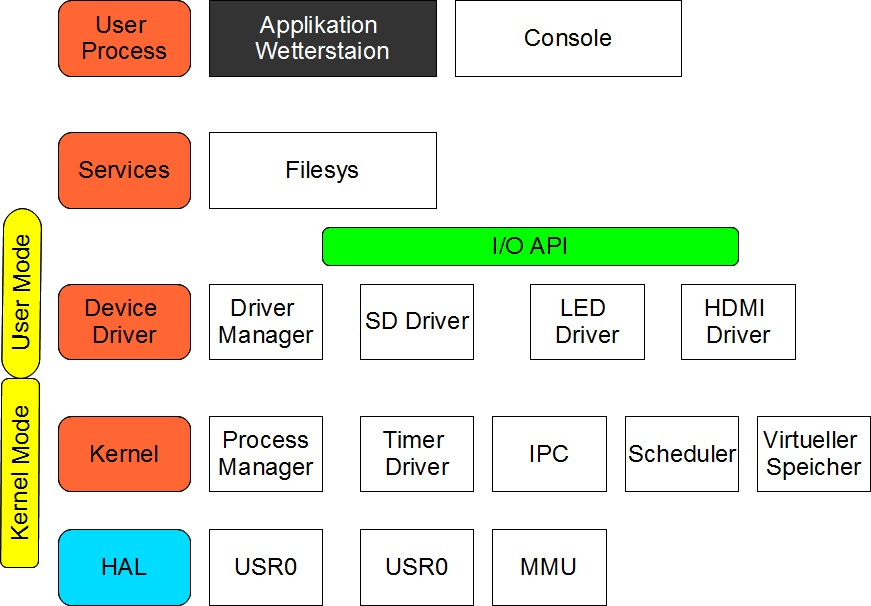
\includegraphics[scale=0.5]{Aufbau/Aufbau.jpg}\linebreak \linebreak
Für das Betriebsystem haben wir uns folgenden Aufbau überlegt.Die oberste Schicht ist der Userprocess, in dem die Wetterapplikation und die Console laufen soll.Darunter liegen die Services z.B Filesys. Dazwischen ist die I/O API. Die nächste Schicht ist die Device Treiber Schicht, in denen befinden sich die ganzen Treiber für die Applikation und das Betriebsystem ( z.B SD Treiber, LED Treiber HDMI Treiber) als auch der Device Manager, der die ganzen Treiber steuert. In der vorletzten Schicht ist der Kernel untegebracht. In dem sitzt der Process manager der den Aufruf und das Beenden der Prozesse steuert.Außerdem noch Timer Driver, IPC, Scheduler, Virtueller Speicher. Die letzte Schicht ist die HAL ( Hardware Abstraction Layer)....


\section{projektspezifische Module}

\subsection{Context switch}
\newpage
\subsection{Interrupts}
\newpage
\subsection{MMU}
	Die Memory Management Unit wurde folgendermaßen implimentiert. Im linkerfile Skript werden die Startaddresse des INT RAM und des EXT DDR definiert. Es werden eine L1 und eine L2 Tabelle verwendet. Die virtuelle Addresse wird folgendermaßen auf eine physikalische Addresse gemappt:\\
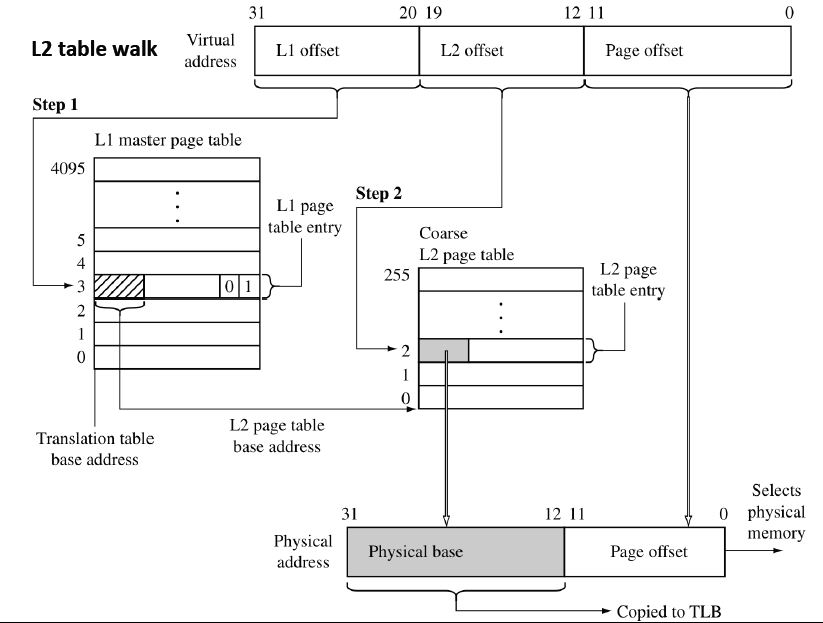
\includegraphics[scale=0.5]{images/VirtuellerSpeicher.png} 

Dabei werden die ersten 3 Hex-Zahlen für den Index in der L1 Tabelle verwendet.Der Inhalt der L1 Tabelle entspricht der Addresse der L2Tabelle. Die nächsten 2 Hex-Zahlen werden für den Index der L2 Tabelle verwendet. In Ihr steht die physikalische Addresse.\\
Für die L1 Tabelle wurden section pages verwendet (1MB) und für die L2 Tabelle wurden small pages (4kB) verwendet.
Interessanter Weise wurde nur 1 Domäne verwendet, deren AP Flags auf 11 gesetzt wurden. Das bedeutet das der man lesen und schreiben darf. Leider konnten wir nicht herausfinden warum andere AP Flags nicht funktionieren. Eigentlich sollten z.B AP Lags wie 01 den Zugriff einschränken und nur im Userprocess lesen dürfen, aber wir hatten keinen Zugriff mehr egal ob User oder Kernel Prozess.\\

Der Kernel wird 1:1 in den INT bzw.EXT DDR RAM gemappt. Die Userprocesse wurden in den EXT DDR gemappt.
\newpage


\subsection{Fat}

\newpage
\subsection{IPC}
\newpage
\subsection{HDMI}
Die Ansteuerung des Bildschirms Liliput 668GL TFT-Monitor wurde durch die Portierung der Grafikschnittstelle von puppybits realisiert.
\newpage
\subsection{I2C}
Nach längere Entwicklungszeit konnten wir den I2C Datenbus nicht auf dem Beagleboard ansteueren. Alle möglichen Fehlerquellen wurden beseitigt, trotzdem konnte der Datenbus nicht angesprochen werden.



\end{document}

